Although the traditional IT security layer provided to Industrial Control Systems offers a great deal of protection, security managers often overlook the possibility of a potential stealthy attacks at the process level. In the paper\supercite{Pasad:2018}, "Truth Will Out: Departure-Based Process-Level Detection of Stealthy Attacks on Control Systems" the authors bring out a novel approach to detecting stealthy attacks on the control system through a process-aware methodology which they call - PASAD. It enables early detection in the subtle variation of process behavior, thus averting strategic adversaries from maliciously manipulating the industrial process within the noise level. The original implementation for the PASAD algorithm was in Matlab. In this replication, I use Python, and popular visualization library, Matplotlib, to obtain the results claimed.

\section*{Introduction}

A typical control system utilizes sensors, actuators, and controllers to regulate some controlled process. Sensor devices measure some physical property and communicate the measurements to a controller (e.g., a PLC), which based on a control algorithm, correspondingly issues commands to actuators
(e.g., control valves) that directly manipulate the physical process based on the received commands. A physical process may exhibit a noisy behavior by nature. A strategic adversary takes advantage of this fact and manipulates the process to stay within the noise level to remain undetected, thus leading to a potential degradation or suboptimal performance or, in the worst scenario, a complete failure of control system through cascading effect between various control loops. PASAD is capable of finding such attacks by utilizing a technique called 'singular spectrum analysis,' a model-free time-series analysis tool.

\section*{Four Steps of PASAD}
Consider a univariate real-valued time series of sensor measurements

\begin{center}
$\mathcal{T}=x_1, x_2,...,x_N, x_N+1$
\end{center}

\subsection*{Step 1: Embedding timeseries data into a trajectory matrix $X$}

Let $L$ be an integer referred to as lag parameter, which is typically close to N/2. Initial $L$ points of $\mathcal{T}$ form the first column vector of Trajectory Matrix $X$. Then the lag vector moves to the next point, similar to the concept of a `moving window' until it covers all the points, forming corresponding column vectors for each. Final trajectory matrix of time series data is as follows:-

$$
X = \begin{bmatrix}
	x_1 & x_2 & \dots  & x_K \\
	x_2 & x_3 & \dots  & x_{K+1} \\
	\vdots & \vdots & \ddots & \vdots \\
	x_L & x_{L+1} & \dots  & x_N
\end{bmatrix}
$$

\subsection*{Step 2: Singular Value Decomposition}


To obtain the noise-reduced version of the above trajectory matrix, we perform singular value decomposition(SVD) on the matrix and obtain the L eigenvectors $u_1, u_2,...,u_L$ and their corresponding eigenvalues. From a scree plot, we determine the cumulative contribution of each eigenvalue to determine the top $r$ contributors to the time series. $r$ represents the statistical dimension, which is the number of degrees of freedom that account for the deterministic variability.

\subsection*{Step 3: Creating a projection matrix}


After obtaining the statistical dimension $r$, we proceed to create the projection matrix. By performing SVD, we have effectively obtained the elementary matrices of $X$ that represents the optimal separation of the component in the trajectory space. Projection  matrix $P$ is obtained through reconstructing/ summing up the top $r$ elementary matrices\supercite{kaggle}. In this step, we also calculate the centroid of this 'reduced' euclidean space and the distance between the centroid and farthest lag vector. This distance is the threshold for determining the anomaly in future lag vectors.

\subsection*{Step 4: Distance Tracking and Anomaly Prediction}

As the lag vector moves forward after completion of threshold distance, we continue projecting lag vectors to the new subspace and see if it is within the threshold distance from the centroid. If yes, it is a usual case, and otherwise, we raise the alarm.

\section*{The Isometry Trick}

The essence of the original paper\supercite{Pasad:2018} is what is called \textbf{the isometry trick}.  In a nutshell, for an arbitrary vector $x$ in $\mathbf{R}^L$, computing the norm of the vector $U^Tx$ has the effect of implicitly projecting $x$ onto the subspace $\mathcal{L}^r$ and computing its norm there. Further reading on the Isometry trick is in Para 2.6 of the original article. By this method, authors have achieved close to linear complexity in the computation, ideal for implementation in low-end devices such as PLCs. 

\section*{Implementation}

The original implementation of PASAD algorithm is in Matlab, and the source code is available \href{https://github.com/mikeliturbe/pasad}{here}. Authors have validated the algorithm with data from three different scenarios namely, The Tennessee-Eastman Process, SWaT Dataset, A Water-Distribution Plant. This reproduction is for the first scenario. Reproduced plots are given below for easy reference.

\subsection*{Scenario 1. (Stealthy Attack)}

Stealthy Attack compromising the control variable XMV(9) detected in sensor variable XMEAS(5). 

\begin{figure}[H]	
	\centering
	\begin{subfigure}[t]{0.45\textwidth}
		\centering
		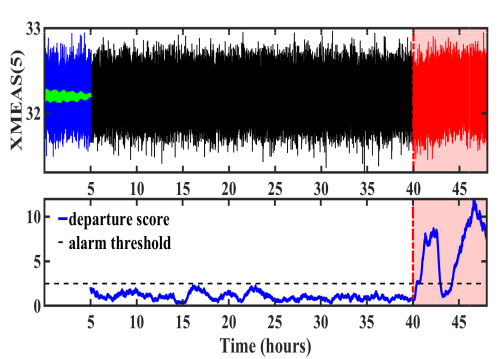
\includegraphics[width=\textwidth]{imgs/sa1orig.png}
		\caption{Original Plot}\label{fig:1a}		
	\end{subfigure}
	\qquad
	\begin{subfigure}[t]{0.45\textwidth}
		\centering
		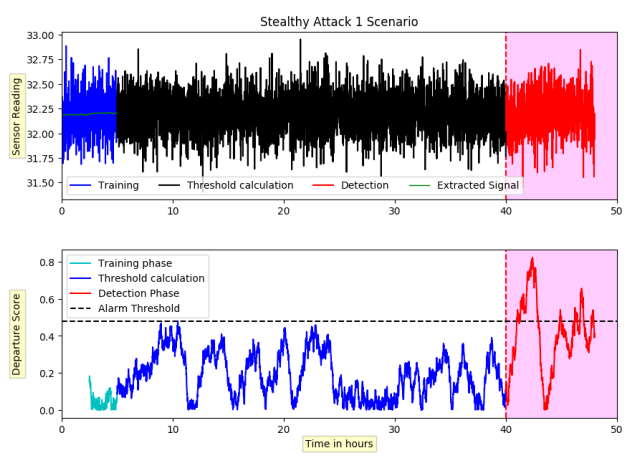
\includegraphics[width=\textwidth]{imgs/sa1re.png}
		\caption{Reproduced plot}\label{fig:1b}
	\end{subfigure}
	\caption{Departure score plot for stealthy attack 1 scenario}\label{fig:1}
\end{figure}

\subsection*{Scenario 2. (Stealthy Attack)}

Stealthy attack SA2 compromising the control variable XMV(6) detected in sensor variable XMEAS(10). 

\begin{figure}[H]	
	\centering
	\begin{subfigure}[t]{0.45\textwidth}
		\centering
		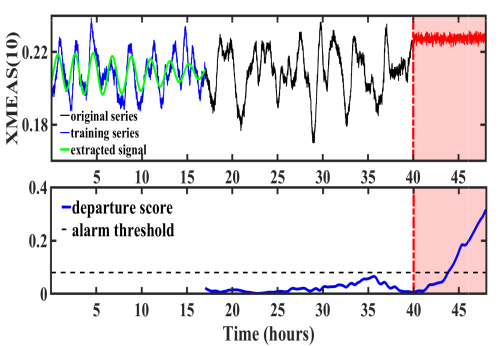
\includegraphics[width=\textwidth]{imgs/sa2orig.png}
		\caption{Original Plot}\label{fig:1a}		
	\end{subfigure}
	\qquad
	\begin{subfigure}[t]{0.45\textwidth}
		\centering
		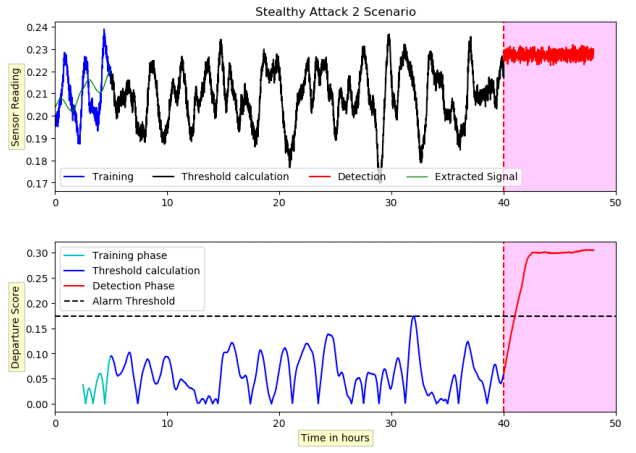
\includegraphics[width=\textwidth]{imgs/sa2re.png}
		\caption{Reproduced plot}\label{fig:1b}
	\end{subfigure}
	\caption{Departure score plot for stealthy attack 2 scenario}\label{fig:1}
\end{figure}

\subsection*{Scenario 3. (Stealthy Attack)}

Stealthy attack SA3 compromising the control variable XMEAS (10) detected in sensor variable XMEAS(9).

\begin{figure}[H]	
	\centering
	\begin{subfigure}[t]{0.45\textwidth}
		\centering
		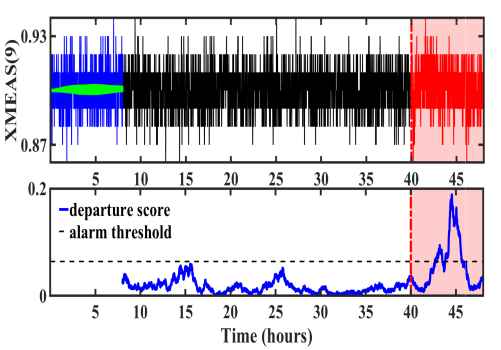
\includegraphics[width=\textwidth]{imgs/sa3orig.png}
		\caption{Original Plot}\label{fig:1a}		
	\end{subfigure}
	\qquad
	\begin{subfigure}[t]{0.45\textwidth}
		\centering
		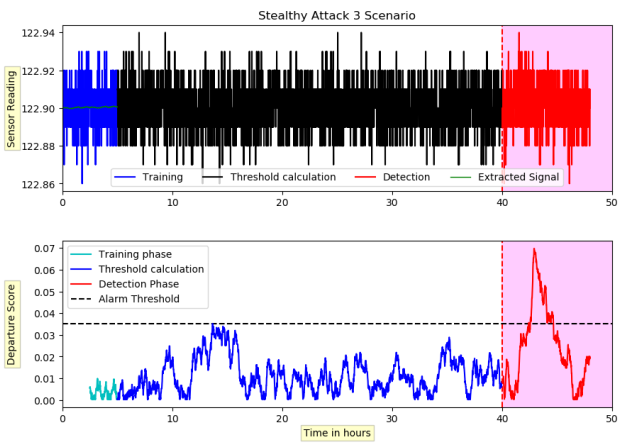
\includegraphics[width=\textwidth]{imgs/sa3re.png}
		\caption{Reproduced plot}\label{fig:1b}
	\end{subfigure}
	\caption{Departure score plot for stealthy attack 3 scenario}\label{fig:1}
\end{figure}

\subsection*{Scenario 4. (Direct Attack)}

Direct Damage attack DA1 compromising the control variable XMV(10) detected in sensor variable XMEAS(15).

\begin{figure}[H]	
	\centering
	\begin{subfigure}[t]{0.45\textwidth}
		\centering
		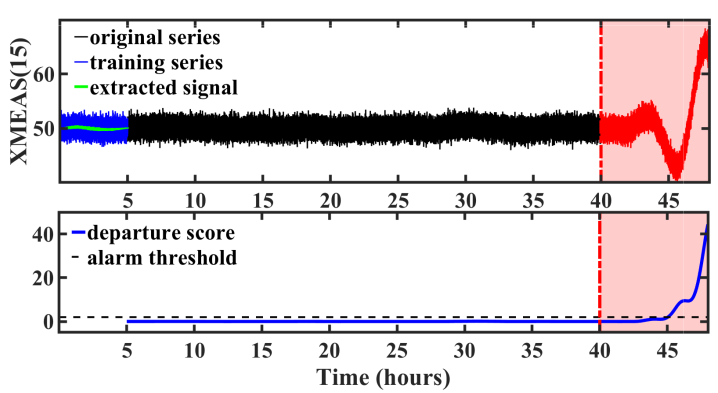
\includegraphics[width=\textwidth]{imgs/da1orig.png}
		\caption{Original Plot}\label{fig:1a}		
	\end{subfigure}
	\qquad
	\begin{subfigure}[t]{0.45\textwidth}
		\centering
		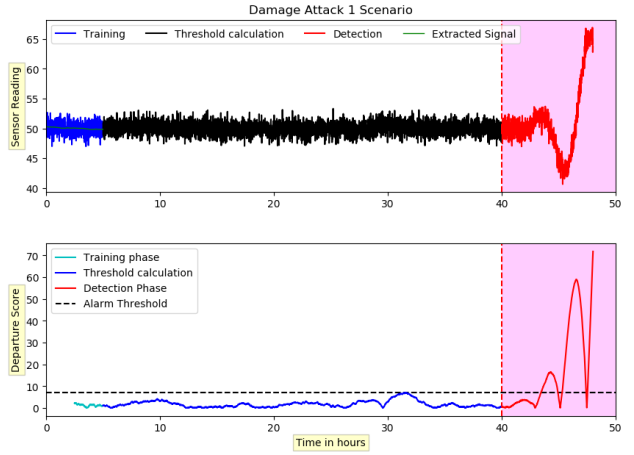
\includegraphics[width=\textwidth]{imgs/da1re.png}
		\caption{Reproduced plot}\label{fig:1b}
	\end{subfigure}
	\caption{Departure score plot for direct attack 1 scenario}\label{fig:1}
\end{figure}

\subsection*{Scenario 5. (Direct Attack)}

Direct Damage attack DA2 compromising the control variable XMEAS(7) detected in sensor variable XMEAS(5). 

\begin{figure}[H]	
	\centering
	\begin{subfigure}[t]{0.45\textwidth}
		\centering
		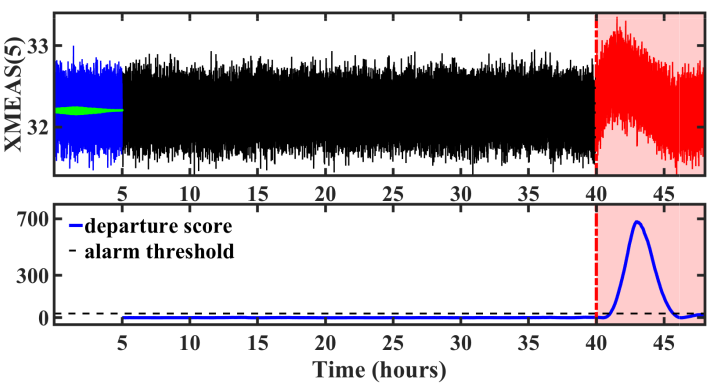
\includegraphics[width=\textwidth]{imgs/da2orig.png}
		\caption{Original Plot}\label{fig:1a}		
	\end{subfigure}
	\qquad
	\begin{subfigure}[t]{0.45\textwidth}
		\centering
		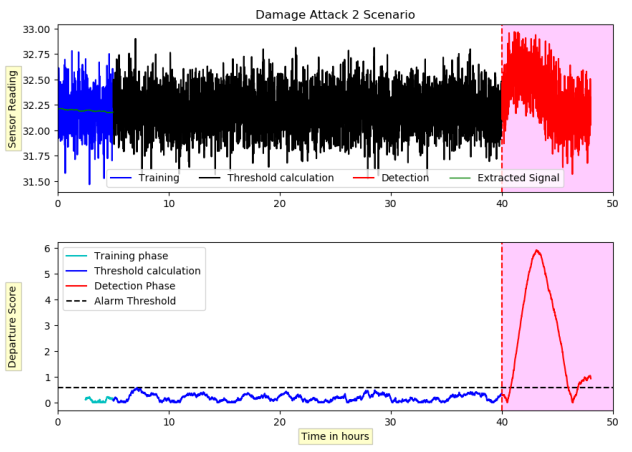
\includegraphics[width=\textwidth]{imgs/da2re.png}
		\caption{Reproduced plot}\label{fig:1b}
	\end{subfigure}
	\caption{Departure score plot for direct attack 2 scenario}\label{fig:1}
\end{figure}


\section*{Results and Observations}
Detection of process manipulations with respect to the 'Tennessee-Eastman Process' dataset, PASAD algorithm was successfully validated. A minor variation in the detection plot is attributable to the selection of statistical dimensions from the scree plot. During reproduction, the first eigenvalue was observed to be disproportionately high due to which the statistical dimensions were selected as 1 to obtain a successful detection phase. The reason for such behavior is attributable to the inherent characteristic of a trajectory matrix, as per clarification by author \href{https://github.com/mikeliturbe/pasad/issues/1}{here}. Variation in screeplot with and without top eigenvalue is as shown in figure \ref{fig:scree}

\begin{figure}[h]	
	\centering
	\begin{subfigure}[t]{0.45\textwidth}
		\centering
		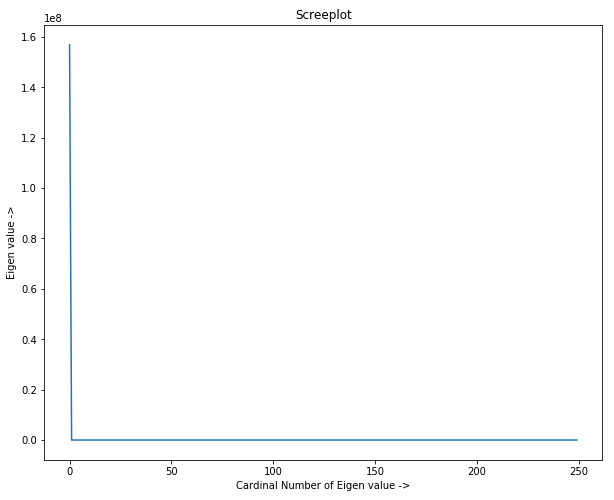
\includegraphics[width=\textwidth]{imgs/scree1.png}
		\caption{All eigenvalues}\label{fig:1a}		
	\end{subfigure}
	\qquad
	\begin{subfigure}[t]{0.45\textwidth}
		\centering
		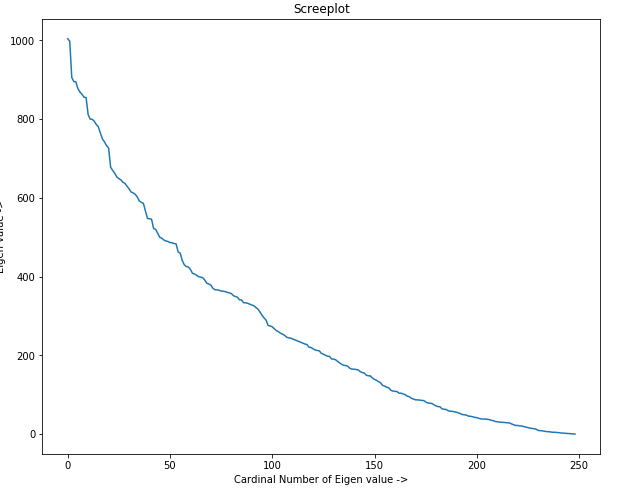
\includegraphics[width=\textwidth]{imgs/scree2.png}
		\caption{Eigenvalues excluding first}\label{fig:1b}
	\end{subfigure}
	\caption{Scree plot of top eigen values}\label{fig:scree}
\end{figure}

\section*{Acknowledgement}

This work is undertaken as part of course CS631A-Cybersecurity for Critical Infrastructure at IIT Kanpur by \href{https://security.cse.iitk.ac.in/node/96}{Prof. Sandeep Shukla}. I would also like to thank \href{https://www.labri.fr/perso/nrougier/}{Nicolas P. Rougier} for letting me know about \href{https://rescience.github.io}{ReScience C} and \href{https://www.cse.iitk.ac.in/users/pvcharan/} {P.V. Sai Charan} for collaborating.
